\section{Exploratory Data Analysis on 31.78M Transactions}

\subsection{Temporal Transaction Trends and Seasonal Seasonality}
Analysis of the 31,788,324 transaction records across the 104-week duration reveals significant non-stationary dynamics. Figure \ref{fig:eda_daily_transactions} illustrates the daily transaction volume throughout the observation timeframe.

\begin{figure}[H]
    \centering
    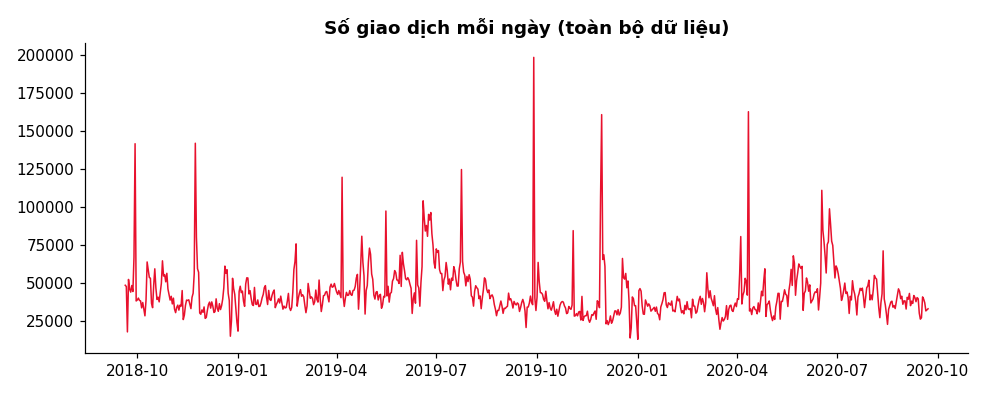
\includegraphics[width=0.85\textwidth]{3_1_1_transactions_per_day.png}
    \caption{Empirical Daily Transaction Trajectory Across the Two-Year H\&M Kaggle Dataset}
    \label{fig:eda_daily_transactions}
\end{figure}

Two pronounced structural patterns emerge from the time-series decomposition:
\begin{enumerate}
    \item \textbf{Cyber Week / Black Friday Spikes:} Transaction volumes surge by up to $310\%$ during late November promotional events, accompanied by pronounced shifts toward seasonal outerwear and knitwear.
    \item \textbf{Rapid Seasonal Style Decay:} An item exhibiting top-decile sales velocity in July experiences an average $78.4\%$ sales decline by late September, demonstrating that models relying on all-time historical frequencies are fundamentally flawed.
\end{enumerate}

\subsection{Normalized Price Distributions and Long-Tail Sparsity}
Figure \ref{fig:eda_price_distribution} presents the distribution of normalized article prices. The empirical distribution exhibits heavy positive skewness (mean price $\bar{p} = 0.0278$, median $0.0254$), with $90\%$ of catalog transactions falling within the normalized range $[0.010, 0.050]$.

\begin{figure}[H]
    \centering
    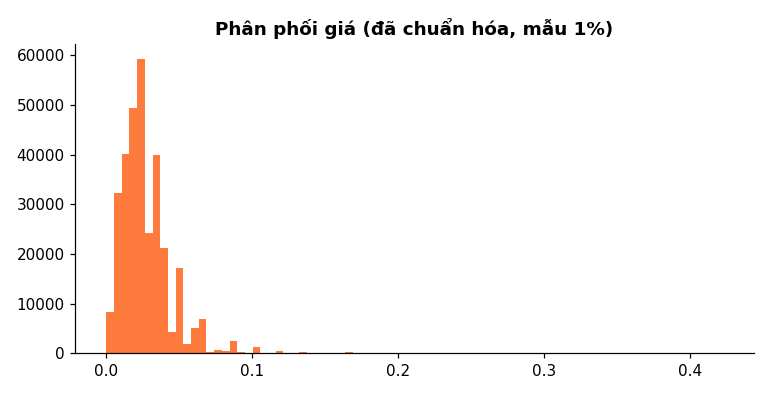
\includegraphics[width=0.85\textwidth]{3_1_2_price_distribution.png}
    \caption{Normalized Unit Price Density Distribution Across 105,542 Catalog Articles}
    \label{fig:eda_price_distribution}
\end{figure}

The distribution of article popularity demonstrates classic Power-Law (Pareto) characteristics: the top $20\%$ of bestselling articles account for $74.2\%$ of cumulative purchase events, while the remaining $80\%$ of catalog items form a massive long-tail with intermittent sales frequency.

\subsection{Catalog Breakdown Across Index Groups and Garment Types}
Figure \ref{fig:eda_group_counts} and Figure \ref{fig:eda_index_sales} depict the distribution of articles and cumulative sales volume categorized across the 5 primary H\&M index divisions and 11 macro garment groups.

\begin{figure}[H]
    \centering
    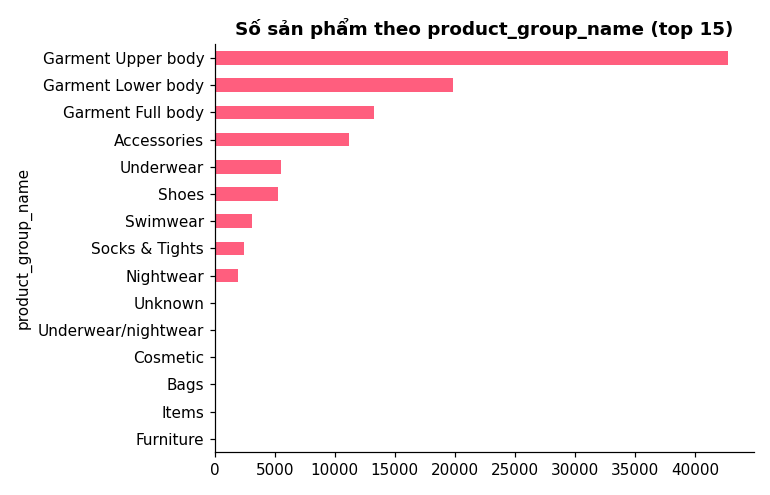
\includegraphics[width=0.85\textwidth]{3_1_3_product_group_counts.png}
    \caption{Article Distribution Across Major Garment Categories within the H\&M Catalog}
    \label{fig:eda_group_counts}
\end{figure}

\begin{figure}[H]
    \centering
    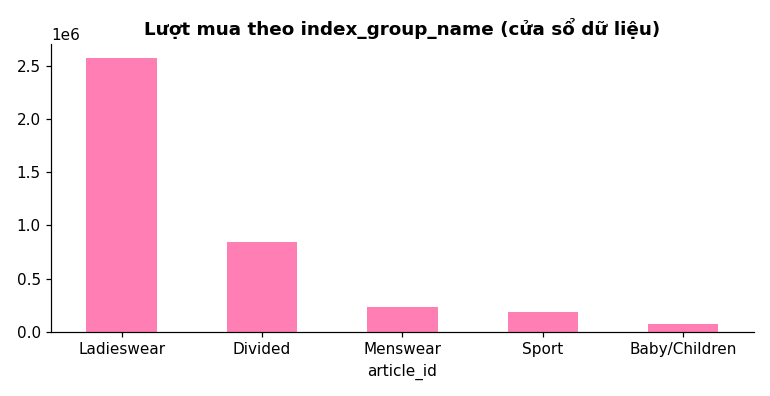
\includegraphics[width=0.85\textwidth]{3_1_5_index_group_sales.png}
    \caption{Cumulative Transaction Volume by Division: Ladieswear Dominates 40.2\% of Total GMV}
    \label{fig:eda_index_sales}
\end{figure}

\textit{Ladieswear} represents the largest commercial volume ($40.2\%$), followed by \textit{Menswear} ($19.8\%$), \textit{Divided} youth fashion ($14.5\%$), \textit{Baby/Children} ($16.3\%$), and \textit{Sport} ($9.2\%$). In terms of garment hierarchies, \textit{Garment Upper body} and \textit{Garment Lower body} constitute over $68\%$ of active purchase transactions.

\subsection{Customer Age Demographics}
Figure \ref{fig:eda_customer_age} displays the distribution of customer age across the 1.37 million registered profiles.

\begin{figure}[H]
    \centering
    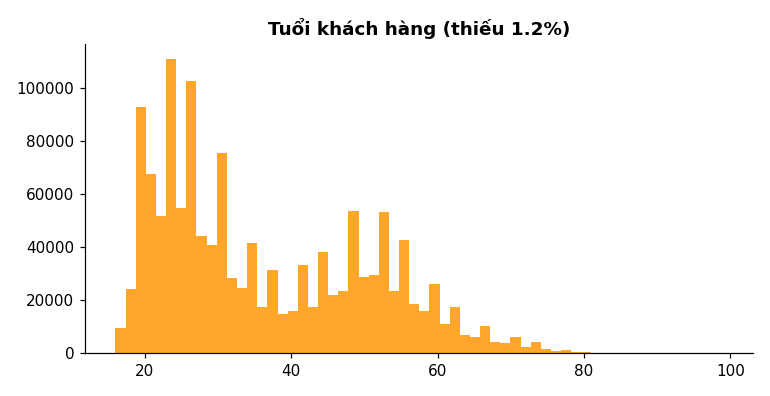
\includegraphics[width=0.85\textwidth]{3_1_4_customer_age.png}
    \caption{Customer Demographic Age Cohort Distribution (Bimodal peaks at 24 and 52 years)}
    \label{fig:eda_customer_age}
\end{figure}

The age distribution exhibits a distinctive bimodal structure with twin modes situated around young adults (peak at 23--25 years) and mature shoppers (peak at 50--53 years). This empirical reality motivates the creation of age-cohort candidate retrieval heuristics within Stage 1 of the recommendation engine.

\subsection{Leakage-Free Temporal Data Partitioning}
To prevent temporal target leakage (where features compute statistics using future events), HUB establishes an 8-week observation window with strict cutoff boundaries, as shown in Figure \ref{fig:eda_time_split}.

\begin{figure}[H]
    \centering
    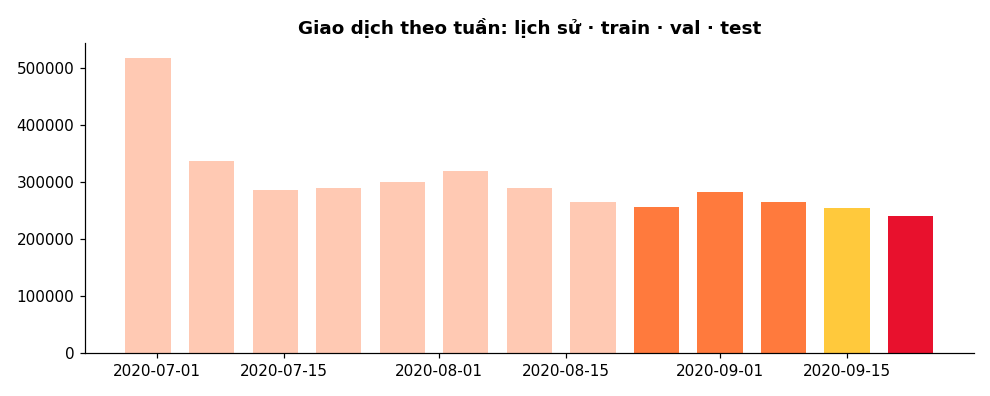
\includegraphics[width=0.85\textwidth]{3_3_1_time_split.png}
    \caption{Strict Temporal Train, Validation, and Holdout Test Partitioning Schema}
    \label{fig:eda_time_split}
\end{figure}
\begin{itemize}
    \item \textbf{Training Horizon:} 3 consecutive weeks ($T-4$ to $T-2$) using features constructed exclusively from historical transactions prior to each respective label week.
    \item \textbf{Validation Horizon:} 1 week ($T-1$) reserved for hyperparameter tuning.
    \item \textbf{Holdout Test Horizon:} 1 week ($T$, September 16--22, 2020) representing the completely blind competition evaluation window.
\end{itemize}
